\section{Observation and Calculations}

\subsection{Recording Scattering Rate as a function of $\theta$}

The counts observed for different values of scattering angles are given in Table \ref{tab}. Using this, we have plotted $\theta$ vs. $N(\theta)$ and have fitted a best-fit plot of the form,

\begin{align} \label{eq:gen}
    f(\theta) = \frac{A}{\sin^4\left(\frac{\theta-B}{2}\right)}
\end{align}

Since the function blows up at $\theta=0$ angle, our analysis focuses on measurements taken in the range $|\theta| > 5^\circ$. The data is plotted along with the best-fit curve according to $f(\theta)$ in Fig. \ref{plot}. The best-fit values of $A$ and $B$ obtained are:

\begin{align*}
    A &= (0.014 \pm 0.006) \text{ s}^{-1}\\
    B &= (-0.026 \pm 0.014)^\circ
\end{align*}

\begin{figure}
    \centering
    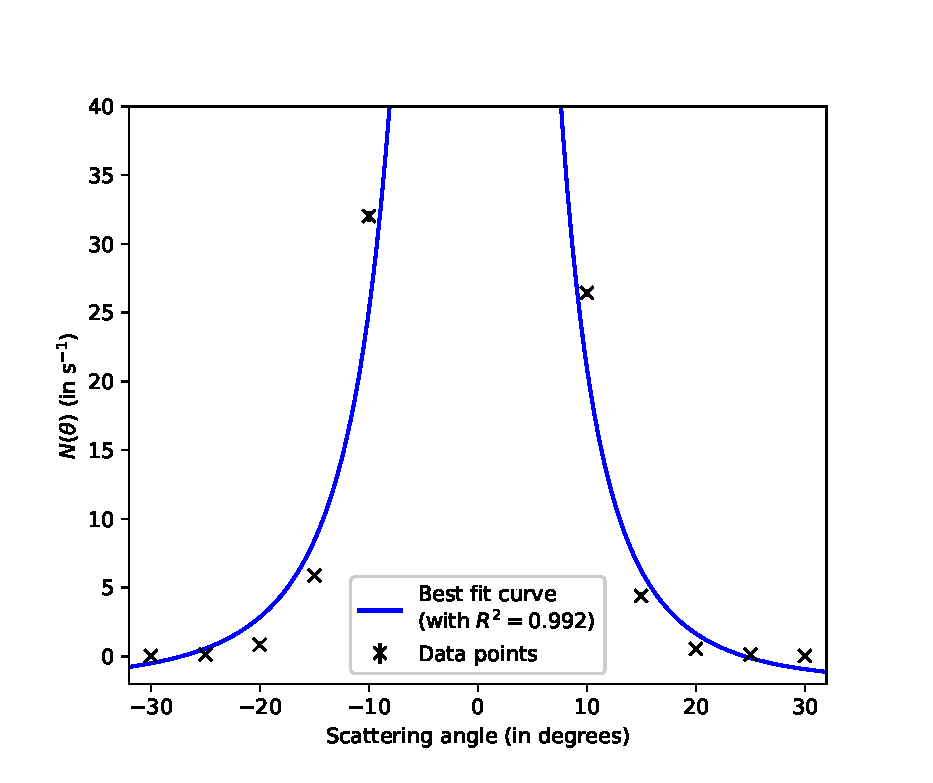
\includegraphics[width=1\columnwidth]{images/plt.eps}
    \caption{$N(\theta)$ vs. scattering angle plot. The standard deviation in $N(\theta)$ is too small to be noticed.}
    \label{plot}
\end{figure}

Hence, we can say that our experiment results validate Rutherford's scattering formula as they roughly obey a $\sin^{-4}(\theta/2)$ relation.

\begin{table}[]
    \centering
    \begin{tabular}{|c|c|c|c|c|c|}
    \hline
    $\theta\,(^\circ)$ & $t(\theta)$ (s) & $n(\theta)$ & $n_\text{avg}(\theta)$ & $N_d(\theta)$ (in s$^{-1}$) & $N(\theta)$ (in s$^{-1}$) \\ \hline
    \multirow{3}{*}{5} & \multirow{3}{*}{100} & 5082 & \multirow{3}{*}{5070.3} & \multirow{3}{*}{50.70} & \multirow{3}{*}{92.59} \\ \cline{3-3}
     &  & 5024 &  &  &  \\ \cline{3-3}
     &  & 5105 &  &  &  \\ \hline
    \multirow{3}{*}{10} & \multirow{3}{*}{100} & 2880 & \multirow{3}{*}{2885.0} & \multirow{3}{*}{28.85} & \multirow{3}{*}{26.44} \\ \cline{3-3}
     &  & 2912 &  &  &  \\ \cline{3-3}
     &  & 2863 &  &  &  \\ \hline
    \multirow{3}{*}{15} & \multirow{3}{*}{100} & 712 & \multirow{3}{*}{714.0} & \multirow{3}{*}{7.14} & \multirow{3}{*}{4.39} \\ \cline{3-3}
     &  & 693 &  &  &  \\ \cline{3-3}
     &  & 737 &  &  &  \\ \hline
    \multirow{3}{*}{20} & \multirow{3}{*}{200} & 220 & \multirow{3}{*}{230.7} & \multirow{3}{*}{1.15} & \multirow{3}{*}{0.54} \\ \cline{3-3}
     &  & 225 &  &  &  \\ \cline{3-3}
     &  & 247 &  &  &  \\ \hline
    \multirow{2}{*}{25} & \multirow{2}{*}{600} & 205 & \multirow{2}{*}{205.0} & \multirow{2}{*}{0.34} & \multirow{2}{*}{0.13} \\ \cline{3-3}
     &  & 205 &  &  &  \\ \hline
    \multirow{2}{*}{30} & \multirow{2}{*}{900} & 127 & \multirow{2}{*}{124.0} & \multirow{2}{*}{0.14} & \multirow{2}{*}{0.04} \\ \cline{3-3}
     &  & 121 &  &  &  \\ \hline
    \multirow{3}{*}{-5} & \multirow{3}{*}{100} & 5295 & \multirow{3}{*}{5278.3} & \multirow{3}{*}{52.78} & \multirow{3}{*}{96.39} \\ \cline{3-3}
     &  & 5281 &  &  &  \\ \cline{3-3}
     &  & 5259 &  &  &  \\ \hline
    \multirow{2}{*}{-10} & \multirow{2}{*}{100} & 3466 & \multirow{2}{*}{3492.0} & \multirow{2}{*}{34.92} & \multirow{2}{*}{32.01} \\ \cline{3-3}
     &  & 3518 &  &  &  \\ \hline
    \multirow{2}{*}{-15} & \multirow{2}{*}{100} & 947 & \multirow{2}{*}{953.5} & \multirow{2}{*}{9.54} & \multirow{2}{*}{5.86} \\ \cline{3-3}
     &  & 960 &  &  &  \\ \hline
    \multirow{2}{*}{-20} & \multirow{2}{*}{200} & 340 & \multirow{2}{*}{368.5} & \multirow{2}{*}{1.84} & \multirow{2}{*}{0.86} \\ \cline{3-3}
     &  & 397 &  &  &  \\ \hline
    \multirow{2}{*}{-25} & \multirow{2}{*}{600} & 252 & \multirow{2}{*}{261.0} & \multirow{2}{*}{0.44} & \multirow{2}{*}{0.16} \\ \cline{3-3}
     &  & 270 &  &  &  \\ \hline
    \multirow{2}{*}{-30} & \multirow{2}{*}{900} & 133 & \multirow{2}{*}{131.0} & \multirow{2}{*}{0.15} & \multirow{2}{*}{0.05} \\ \cline{3-3}
     &  & 129 &  &  &  \\ \hline
    \end{tabular}
    \caption{Measured counts $n$ for different scattering angles for Au foil of width 5mm. $N_d$ refers to counts per second. $N$ refers to the space corrected count rate as per Eq. \ref{eq:4}.}
    \label{tab}
    \end{table}

\subsection{Determination of the atomic number of Aluminium}
The count rates for Au and Al foils of slit width 1mm are given in Table \ref{tab:z}. The following parameters are known to us:

\begin{itemize}
    \item Thickness of the gold foil, $d_\text{Au} = 2\mu$m
    \item Thickness of the aluminium foil, $d_\text{Al} = 8\mu$m
    \item Atomic concentration approximation, $c_\text{Al} = c_\text{Au}$
    \item Nuclear charge of gold, $Z_\text{Au} = 79$
    \item Slit width (for both Au and Al) $ = 1$ mm.
\end{itemize}

\noindent Using Eq. \ref{eq:part2}, we can plug in the above values to get,

\begin{align*}
    \implies Z_\text{Al} = 79\sqrt{\frac{2\cdot 0.320}{8 \cdot 0.0325}} = 12.6
\end{align*}

\begin{table}[]
    \centering
    \begin{tabular}{|c|c|c|c|c|c|}
    \hline
    Material & $\theta\,(^\circ)$ & $t(\theta)$ (s) & $n(\theta)$ & $n_\text{avg}(\theta)$ & $N_d(\theta)$ (in s$^{-1}$) \\ \hline
    \multirow{8}{*}{Au} & \multirow{4}{*}{-15} & \multirow{8}{*}{100} & 45 & \multirow{8}{*}{32.0} & \multirow{8}{*}{0.320} \\ \cline{4-4}
     &  &  & 35 &  &  \\ \cline{4-4}
     &  &  & 26 &  &  \\ \cline{4-4}
     &  &  & 27 &  &  \\ \cline{2-2} \cline{4-4}
     & \multirow{4}{*}{15} &  & 27 &  &  \\ \cline{4-4}
     &  &  & 30 &  &  \\ \cline{4-4}
     &  &  & 30 &  &  \\ \cline{4-4}
     &  &  & 36 &  &  \\ \hline
    \multirow{4}{*}{Al} & \multirow{2}{*}{-15} & \multirow{4}{*}{1000} & 30 & \multirow{4}{*}{32.5} & \multirow{4}{*}{0.033} \\ \cline{4-4}
     &  &  & 29 &  &  \\ \cline{2-2} \cline{4-4}
     & \multirow{2}{*}{15} &  & 26 &  &  \\ \cline{4-4}
     &  &  & 45 &  &  \\ \hline
    \end{tabular}
    \caption{Measured count rates for Au and Al foils of slit width 1mm}
    \label{tab:z}
    \end{table}
\section{Error analysis}

From Eq. \ref{eq:part2}, we can get the uncertainity in $N_\text{Al}$ as, 

\begin{align}
    \frac{\Delta Z_\text{Al}}{Z_\text{Al}} = \sqrt{\left(\frac{\Delta N_\text{Au}}{2N_\text{Au}}\right)^2+\left(\frac{\Delta N_\text{Al}}{2N_\text{Al}}\right)^2+\left(\frac{\Delta d_\text{Au}}{2d_\text{Au}}\right)^2\left(\frac{\Delta d_\text{Al}}{2d_\text{Al}}\right)^2}
\end{align}

By assuming $\Delta d=0$ and taking the $\Delta N$ values as the standard deviation in count rates we have $\Delta N_\text{Al} = 7.37/1000s = 7.37 \times 10^{-3}$ s$^{-1}$ and $\Delta N_\text{Al}= 6.00/100s = 6.00 \times 10^{-2}$ s$^{-1}$,

\begin{align*}
    \Delta Z_\text{Al} = 1.8
\end{align*}
